\documentclass[12pt]{amsart}
\usepackage{latexsym}
\usepackage{amssymb,amsmath}
\usepackage[pdftex]{graphicx}
\usepackage{enumerate}
\usepackage{endnotes}
%\usepackage{extpfeil}
\usepackage{hyperref}
\usepackage[usenames,dvipsnames]{xcolor}
\usepackage{stackrel}
\usepackage{bbm}
\usepackage{tikz}
\usepackage[margin=1.25in]{geometry}
\usepackage{hyperref}
\usepackage{listings}
\usepackage{courier}
\usepackage{color}
\usepackage{upgreek}

\lstset{
	basicstyle=\small\ttfamily,
	keywordstyle=\color{blue},
	language=python,
	xleftmargin=16pt,
}

\usetikzlibrary{arrows,chains,matrix,positioning,scopes}

\makeatletter
\tikzset{join/.code=\tikzset{after node path={%
\ifx\tikzchainprevious\pgfutil@empty\else(\tikzchainprevious)%
edge[every join]#1(\tikzchaincurrent)\fi}}}
\makeatother
%
\tikzset{>=stealth',every on chain/.append style={join},
         every join/.style={->}}
\tikzstyle{labeled}=[execute at begin node=$\scriptstyle,
   execute at end node=$]
\usetikzlibrary{patterns}

\usetikzlibrary{decorations.pathreplacing}

\DeclareSymbolFont{bbold}{U}{bbold}{m}{n}
\DeclareSymbolFontAlphabet{\mathbbold}{bbold}

\newtheorem{thm}{Theorem}[section]
\newtheorem{ithm}{Theorem}
\newtheorem{lem}[thm]{Lemma}
\newtheorem{conj}[thm]{Conjecture}
\newtheorem{prop}[thm]{Proposition}
\newtheorem{cor}[thm]{Corollary}

\theoremstyle{definition}
\newtheorem{defi}[thm]{Definition}
\newtheorem{example}[thm]{Example}
\newtheorem{exercise}[thm]{Exercise}
\newtheorem{rem}[thm]{Remark}


   
\def\B{{\mathbb B}}
\def\C{{\mathbb C}}
\def\D{{\mathbb D}}
\def\Fp{{\mathbb F}_p}
\def\Fell{{\mathbb F}_{\ell}}
\def\F{{\mathbb F}}
\def\H{{\mathbb H}}
\def\M{{\mathbb M}}
\def\N{{\mathbb N}}
\def\O{{\mathcal O}}
\def\0{{\mathbb 0}}
\def\P{{{\mathbb P}}}
\def\Q{{\mathbb Q}}
\def\R{{\mathbb R}}
\def\T{{\mathbb T}}
\def\Z{{\mathbb Z}}

\newcommand{\sol}{_{a^p,b^p,c^p}}
\newcommand{\bound}{\partial}
\newcommand{\la}[1]{\mathfrak{#1}}
\newcommand{\im}{\text{Im} \hspace{0.1em} }
\newcommand{\ann}{\text{Ann} \hspace{0.1em} }
\newcommand{\rank}{\text{rank} \hspace{0.1em} }
\newcommand{\coker}[1]{\text{coker}\hspace{0.1em}{#1}}
\newcommand{\sgn}{\text{sgn}}
\newcommand{\lcm}{\text{lcm}}
\newcommand{\re}{\text{Re}  \hspace{0.1em} }
\newcommand{\ext}[1]{\text{Ext}(#1)}
\newcommand{\Hom}[1]{\text{Hom}(#1)}
\newcommand{\End}[1]{\text{End(#1)}}
\newcommand{\bs}{\setminus}
\newcommand{\rpp}[1]{\mathbb{R}\text{P}^{#1}}
\newcommand{\cpp}[1]{\mathbb{C}\text{P}^{#1}}
\newcommand{\tr}{\text{tr}\hspace{0.1em} }
\newcommand{\inner}[1]{\langle {#1}\rangle}
\newcommand{\tensor}{\otimes}
\newcommand{\Cl}{\text{Cl}}
\renewcommand{\sp}[1]{\text{Sp}_{#1}}
\newcommand{\GL}{\text{GL}}
\newcommand{\PGL}{\text{PGL}}
\renewcommand{\sl}[1]{\text{SL}_{#1}}
\newcommand{\so}[1]{\text{SO}_{#1}}
\newcommand{\SO}{\text{SO}}
\newcommand{\pso}[1]{\text{PSO}_{#1}}
\renewcommand{\o}[1]{\text{O}_{#1}}
\renewcommand{\sp}[1]{\text{Sp}_{#1}}
\newcommand{\psp}[1]{\text{PSp}_{#1}}
\newcommand{\Span}{\rm Span}
\newcommand{\Frob}{\rm Frob}
\newcommand{\tor}{\rm tor}
\newcommand{\rad}{\rm rad}
\newcommand{\denom}{\rm denom}
\renewcommand{\bar}{\overline}
\newcommand{\notdiv}{\nmid}
\newcommand{\pfrac}[2]{\left( \frac{#1}{#2} \right)}
\newcommand{\bfrac}[2]{\left| \frac{#1}{#2} \right|}
\newcommand{\Ell}{\rm Ell}
\newcommand{\AV}{\rm AV}
\newcommand{\Gal}{\rm Gal}

\newcommand{\kron}[2]{\bigl(\frac{#1}{#2}\bigr)}
\newcommand{\leg}[2]{\Biggl(\frac{#1}{#2}\Biggr)}

\DeclareSymbolFont{bbold}{U}{bbold}{m}{n}
\DeclareSymbolFontAlphabet{\mathbbold}{bbold}

\begin{document}

\title{Perfect Powers in Lucas Sequences via Galois Representations}
\author{Jesse Silliman and Isabel Vogt}

\maketitle


\section{Preliminaries}

Let $(b,c)$ define the linear binary recurrence relation.
\[ u_{n+2} = b\cdot u_{n+1}+ c\cdot u_n. \]
with characteristic polynomial with roots
\[ g(z) = z^2 - bz - c, \qquad \qquad \alpha, \beta = \frac{b \pm \sqrt{b^2+4c}}{2}.\]

We will be primarily interested in the companion sequences for a given recurrence relation $(b,c)$, refered to as $u_n$ and $v_n$, specified by the starting conditions
\[ u_0 = 0, u_1 = 1 \qquad \qquad v_0 = 2, v_1 = b \]
The $n$th terms of these sequence are specified by the formulas
\[u_n = \frac{\alpha^n - \beta^n}{\alpha - \beta} \qquad \qquad v_n = \alpha^n +\beta^n \]
It is straightforward to verify the following facts
\begin{equation}\label{fib2} u_{2k} = u_kv_k \end{equation}
\begin{equation}\label{gen_diophan}(\alpha - \beta)^2u_n^2 = v_n^2 - 4(\alpha\beta)^n \end{equation}
The second fact in the list allows us to generate Frey curves.  In particular, say that we posit a solution $u_n = y^p$, that is
\begin{equation}\label{rel_diophan} (b^2+4c)y^{2p}+4(-c)^n = v_n^2 .\end{equation}
This is a solution to the $(p,p,2)$-with-coefficients Diophantine equation
\[ (b^2+4c)X^p +4(-c)^nY^p = Z^2. \]

Using \cite{bennett04} we associate a \textit{primitive} solution to an elliptic curve (a Frey curve) in such a way that the discriminant and conductor of our Frey curve take a particularly simple form by virtue of the solution to the Diophantine equation.  For any such recurrence relation (with $\gcd(b,c)=1$) we choose Frey curves with discriminant and conductor in the following way.

\begin{prop}\label{freycurves}
Assume $u_n = y^p$ for $p,n \geq 5$.  We may write the associated Diophantine equation as
\[ (b^2+4c)y^{2p} + 4(-c)^n = z^2.\]
As a convention let $k_1 = \upnu_2(b^2+4c)$, $k_2 = \upnu_2(y^{2p})$, and $k = k_1+k_2$.  Without loss of generality we may assume that we are in one of the following situations:

\begin{enumerate}[1.]

\item $b,c$ relatively prime

\begin{enumerate}[(i)]

\item $b^2+4c \equiv 1 \pmod{4}$, and $2 \notdiv y,z,c$, and $z \equiv -(-c)^n \pmod{4}$.
\[ E_i: Y^2 = X^3 + zX^2 + (-c)^nX \]
\[ \Delta = 2^4(-c)^{2n}(b^2+4c)y^{2p},  \qquad N = 2^{\alpha} \prod_{\substack{ \ell | 2c \cdot (b^2+4c) \\ \ell | y}} \ell, \qquad \alpha =  \begin{cases} 1: (-c)^n \equiv -1 \pmod{4}\\ 2 : (-c)^n \equiv 1 \pmod{4} \end{cases} \]
\item $b^2+4c \equiv 1 \pmod{4}$, $2|y,z$, $2 \notdiv c$, let $y = 2\hat{y}, z = 2\hat{z}$, with $\hat{z} \equiv 1 \pmod{4}$.
\[ E_{ii} : Y^2 +XY = X^3 + \frac{\hat{z} - 1}{4} X^2 + (b^2+4c)2^{2p-8}\hat{y}^{2p}X \]
\[ \Delta = 2^{2p-14}(b^2+4c)^2(-c)^ny^{4p}, \qquad N = \prod_{\substack{ \ell | c \cdot (b^2+4c) \\ \ell | y}} \ell  \]
\item $b^2+4c \equiv 1 \pmod{4}$, $2|c$, $2 \notdiv y,z$, and $z \equiv 1 \pmod{4}$
\[ E_{iii}: Y^2 +XY = X^3 +\frac{z-1}{4}X^2 +2^{-4}(-c)^nX \]
\[ \Delta = 2^{-8}(-c)^{2n}(b^2+4c)y^{2p} , \qquad N = \prod_{\substack{ \ell | c \cdot (b^2+4c) \\ \ell | y}} \ell  \]
\item $k = 2$, $z = 2 \hat{z}, y = 2^{2pk_2}\hat{y}^{2p}$, $(b^2+4c) = 2^{k_1}D$
\[D \equiv -1 \pmod{4} \qquad \qquad E_{iv} : Y^2 = X^3 +2\hat{z}X^2 +D\hat{y}^{2p}X \]
\[\Delta = 2^{6}D^2(-c)^n\hat{y}^{2p}, \qquad \qquad N = 2^{5}\prod_{\substack{ \ell | c \cdot D \\ \ell | \hat{y}}} \ell  \]

\[D \equiv \ \ 1 \pmod{4}  \qquad \qquad  E_{iv} : Y^2 = X^3 +2\hat{z}X^2 +(-c)^nX \]
\[\Delta = 2^{6}D(-c)^{2n}\hat{y}^{2p}, \qquad \qquad N = 2^{5}\prod_{\substack{ \ell | c \cdot D \\ \ell | \hat{y}}} \ell  \]

\item $k = 3$, $z = 2 \hat{z}, y = 2^{2pk_2}\hat{y}^{2p}$, $(b^2+4c) = 2^{k_1}D$
\[ E_{v} : Y^2 = X^3 + 2\hat{z}X^2 + 2D\hat{y}^{2p}X \]
\[ \Delta = 2^8D^2(-c)^n\hat{y}^{4p} , \qquad \qquad N = 2^6 \prod_{\substack{ \ell | c \cdot 2D \\ \ell | \hat{y}}} \ell  \]

\item $k=4$, $z = 2 \hat{z}, y = 2^{2pk_2}\hat{y}^{2p}$, $(b^2+4c) = 2^{k_1}D$ with $\hat{z} \equiv -D \pmod{4}$
\[ E_{vi} : Y^2 = X^3 +\hat{z}X^2 + D \hat{y}^{2p} X \]
\[ \Delta = 2^4D^2(-c)^n\hat{y}^{4p}, \qquad N = 2^\alpha \prod_{\substack{ \ell | c \cdot 2D \\ \ell | \hat{y}}} \ell ,  \qquad \alpha =  \begin{cases} 1: D \equiv -1 \pmod{4}\\ 2 : D \equiv 1 \pmod{4} \end{cases} \]


\item $k = 5,6,7$, $z = 2 \hat{z}, y = 2^{2pk_2}\hat{y}^{2p}$, $(b^2+4c) = 2^{k_1}D$ with $\hat{z} \equiv 1 \pmod{4}$
\[ E_{vii} : Y^2 = X^3 + \hat{z}X^2 + 2^{k-4}D \hat{y}^{2p} X \]
\[ \Delta = 2^{2k-4}D^2(-c)^n\hat{y}^{4p}, \qquad N = 2^\alpha \prod_{\substack{ \ell | c \cdot 2D \\ \ell | \hat{y}}} \ell ,  \qquad \alpha =  \begin{cases} 1: k = 5 \\ 2 : k = 6,7 \end{cases} \]

\item $k\geq 8$, $z = 2 \hat{z}, y = 2^{2pk_2}\hat{y}^{2p}$, $(b^2+4c) = 2^{k_1}D$ with $\hat{z} \equiv 1 \pmod{4}$
\[ E_{viii} : Y^2 + XY = X^3 + \frac{\hat{z}-1}{4} X^2 + 2^{k-8}D \hat{y}^{2p} X \]
\[ \Delta = 2^{2k-16}D^2(-c)^n\hat{y}^{4p}, \qquad N = 2^\alpha \prod_{\substack{ \ell | c \cdot 2D \\ \ell | \hat{y}}} \ell ,  \qquad \alpha =  \begin{cases} -1: k = 8 \\ 0 : k > 8 \end{cases} \]


\end{enumerate}

\end{enumerate}
\end{prop}
\begin{proof}
See \cite{bennett04}.  Note that if $c \neq 1$, then $c \notdiv y$ by induction on the recurrence relation.
\end{proof}

To these Frey curves we associate the mod $p$ Galois representation
\[ \rho_{E,p}: G_{\Q} \rightarrow \GL_2(\F_p) \]
corresponding to the $p$-torsion number field $\Q(E[p])$.

\begin{lem}\label{unram}
The mod $p$ Galois representation $\rho_{E,p}$ associated to one of the above Frey curves is unramified at any odd prime $\ell$ not dividing $c \cdot (b^2+4c)$.  Further it is flat at $p$ if $p \notdiv 2c\cdot (b^2+4c)$.
\end{lem}
\begin{proof}
By the N\'{e}ron-Ogg-Shafarevich criterion, the mod $p$ Galois representation is unramified outside $pN_E$.  By the theory of Tate curves, $E(\bar{\Q}_\ell) \simeq \bar{\Q}_\ell^\ast / q^{\Z}$ with $E[p](\bar{\Q}_\ell) = \langle \zeta_p, q^{1/p} \rangle$, so in particular the ramification comes from primes $\ell$ ramified in $\Q(\zeta_p)$ and those such that $p \notdiv \upnu_\ell(q) = \upnu_\ell(\Delta)$.  If $\ell | y$, then as $p \mid \upnu_\ell(\Delta)$, $\rho_{E,p}$ is unramified at $\ell$.  Further as $\Q(\zeta_p) \subset \Q(E[p])$, $\rho_{E,p}$ will be ramified at $p$; however, if $p \mid N$, but $p \notdiv 2c \cdot (b^2+4c)$, then $p \mid y$, and the above argument shows this does not contribute to the ramification.
\end{proof}

Galois representations are particularly useful because of the following two influential theorems of \cite{wiles95}, \cite{taylorwiles95}, \cite{conrad01} and \cite{ribet91}  on the modularity of elliptic curves and level lowering.

\begin{thm}[Modularity of Elliptic Curves \cite{wiles95}, \cite{taylorwiles95}, \cite{conrad01}]\label{modularity}
Let $E$ be an elliptic curve with conductor $N$.  For any prime $p$, there exists a weight 2 newform $f \in S_2(\Gamma_0(N))$ such that
\[ \rho_{E,p} \simeq \bar{\rho_{f,p}} \]
for $\rho_{f,p}$ the 2-dimensional $p$-adic Galois representation of $f$ and $\bar{\rho_{f,p}}$ the reduction of $\rho_{f,p}$ mod $p$.
\end{thm}

\begin{thm}[Level Lowering \cite{ribet91}]\label{levellow}
Let $f$ be a newform of level $\ell N$ with absolutely irreducible 2-dimensional mod $p$ Galois representation $\bar{\rho_{f,p}}$ unramified at $\ell$ if $\ell \neq p$ and flat at $\ell = p$.  Then there exists a weight 2 newform $g$ of level $N$ such that
\[ \bar{\rho_{f,p}} \simeq \bar{\rho_{g,p}}. \]
\end{thm}

The remaining sections of the paper apply these deep theorems to the Frey curves generated from binary recurrence relations to prove nonexistence theorems in a similar style to \cite{siksek06}, \cite{siksek05}.



\section{Results for Specific Sequences}

We now demonstrate the feasibility of these methods to sharply bound $p$ and determine all perfect powers in a recurrence sequence.  We prove both conditional and unconditional bounds in this way. 

We first deal with several examples where $b^2+4c = 1$.

\begin{thm}\label{noforms1}
Let $u_n$ be the binary recursion sequence defined by 
\[ u_{n+2} = bu_{n+1} +cu_n \]
with $b^2+4c = 1$ and initial conditions $u_0 = 0$ and $u_1=1$.  Then for the following values of $b$ and $c$:
\begin{center}
\begin{tabular}{c | c }
b & c \\  \hline \hline
3 & -2 \\
5 & -6  \\
7 & -12 \\
17 & -72  \\
9 & -20 \\ \hline \hline
\end{tabular}
\end{center}
$u_n$ has no nontrivial $p$th powers. %except perhaps for 5th powers in $(9,-20)$.
\end{thm}

In order to prove the above theorem we first establish the following lemmas.

\begin{lem}\label{relprime}
Let $b^2+4c=1$.  For $n \geq 1$,  $u_n$, $v_n$, and $c$ are relatively prime.
\end{lem}

\begin{proof}
We prove this by induction.  First note that $b^2 +4c = 1$ forces $b$ and $c$ to be relatively prime and $c$ to be even.  Clearly as
\[ u_2 = b \cdot u_1 + c \cdot u_0 \]
and $u_1$ is relatively prime to $c$, $u_2$ is relatively prime to $c$.  Thus by induction $u_n$ is relatively prime to $c$.  Similarly for $v_n$.  And further as $u_n^2  = v_n^2 - 4(-c)^n$, no primes except perhaps those dividing $c$ can divide $u_n$ and $v_n$.  Thus they are pairwise relatively prime.
\end{proof}

\begin{lem}[Ruling out small primes]\label{smallp}
There are no nontrivial squares or cube terms in any of the above examples except $u_2 = 9$ for the sequence $(9,-20)$.
\end{lem}

\begin{proof}

We first deal with the case of $p=2$; we will derive our contradiction from the relation \eqref{gen_diophan}, which in this case reduces to
\begin{equation}\label{D1dio} \frac{\alpha^n - (\alpha-1)^n}{1} = z^2.\end{equation} 
Assume that the index $n$, for which $u_n = z^2$, is odd; in this case we can absorb the sign and have a nontrivial integral solution to
\begin{equation}\label{diophanpp2}
x^n +y^n = z^2
\end{equation}
But there are no nontrivial solutions to \eqref{diophanpp2} for $n \geq 4$ by the solution to $(n,n,2)$ in \cite{darmon97} .  We easily check that in our examples, there are no solutions for $n=3$.  In the case $n$ is even, write $n=2^rk$ for $k$ odd.  Then we can write
\begin{align*}
\alpha^{2^rk} - \beta^{2^rk} & = (\alpha^{2^{r-1}k} - \beta^{2^{r-1}k})(\alpha^{2^{r-1}k} + \beta^{2^{r-1}k}) \\
& = (\alpha^{2^{r-1}k} + \beta^{2^{r-1}k})(\alpha^{2^{r-2}k} + \beta^{2^{r-2}k}) \cdots (\alpha^{k} - \beta^{k}) (\alpha^{k} + \beta^{k}). 
\end{align*}
Further by lemma \ref{relprime}, we know that that these terms are relatively prime.  Thus $u_n=z^2$ if and only if each of these terms is also a square.  In particular, $\alpha^k + \beta^k$ must be a square.  If $k \neq 1$, then this is identical to the previous condition, which yields a contradiction.  If $k = 1$, then this is the condition that $b$ is a perfect square.  It is easy to verify that this is not true in all of the above examples, except $(9,-20)$.  Further, $u_2 = 3^3$ is the only square in the sequence $(9,-20)$ as $u_4 = 369$ which is not a square.  The proof for $p=3$ follows in exactly the same way from reduction to odd index and the solution of $(n,n,3)$ by \cite{darmon97}.

\end{proof}

\begin{lem}\label{5irr}
If $E$ is an elliptic curve with $\Delta_E$ a perfect square, then $\rho_{E,5} $ is absolutely irreducible.
\end{lem}
\begin{proof}
If $\rho_{E,5}$ were reducible, it would give rise to a rational point on $X_0(5) \simeq \P_1$.  Let $X_{\Delta} \simeq \P_1$ be the degree $2$ cover of $X(1)$ parameterizing an elliptic curve $E'$ and a choice of square root of its discriminant $\Delta_{E'}$.  The map to $X(1)$ is given by
\[z \mapsto z^2 + 12^3. \]
As $\Delta_E$ is a rational square, $E$ gives rise to a rational point on $X_{\Delta}$.
As in \cite{brown12} we construct the following diagram
\begin{center}
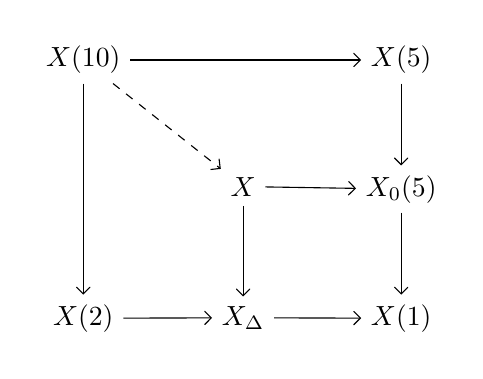
\begin{tikzpicture}[scale=2]
\matrix (m) [matrix of math nodes, row sep=3em, column sep=3em]
{ X(10) & & X(5)  \\
 & X & X_0(5)  \\
X(2) & X_{\Delta} & X(1)\\};
\path[->,font=\scriptsize,>=angle 90]
(m-1-1) edge  (m-3-1)
(m-1-1) edge (m-1-3)
(m-1-3) edge  (m-2-3)
(m-1-1) edge[dashed]  (m-2-2)
(m-2-3) edge  (m-3-3)
(m-2-2) edge  (m-2-3)
(m-2-2) edge  (m-3-2)
(m-3-1) edge  (m-3-2)
(m-3-2) edge  (m-3-3);
\end{tikzpicture}
\end{center}
where $X$ is the normalization of the fiber product $X_{\Delta} \times_{X(1)} X_0(5)$.  $X$ is an elliptic curve given by the equation
\[X: \qquad  y^2 = x^3 + 22x^2 +125x .\]
The map to $X_{\Delta}$ is given by
\[ (x,y) \mapsto \frac{y(x^2-500x -15625)}{x^3}. \]
Sage easily determines that $X$ is rank $0$, with rational point $(0:0:1)$ and $(0:1:0)$, both lying in the kernel of the map to $X_{\Delta}$.  Thus our elliptic curve cannot give rise to a rational point on $X_0(5)$, and we conclude that $\rho_{E,5}$ is irreducible.  Further, irreducible implies absolutely irreducible as $\det: G_\Q \rightarrow \F_p^*$ is the cyclotomic character $\chi_p$ and $\chi_p(c)=-1$ for $c$ complex conjugation.
\end{proof}
\begin{cor}\label{frey5irr}
Let $E$ be a Frey curve arising from a solution $u_n = y^5$ for $b^2+4c = 1$ and $n\geq 5$, then $\rho_{E,5}$ is absolutely irreducible.
\end{cor}
\begin{proof}
By proposition \ref{freycurves} all of the discriminants of these Frey curves are rational squares.
\end{proof}


\begin{proof}[Proof of Theorem \ref{noforms1}]
Posit a solution $u_n = y^p$ for $n \geq 5$ and $p \geq 5$.  We have a Diophantine equation
\[ y^{2p} + 4(-c)^n = v_n^2. \] 
By lemma \ref{relprime} the solution $(y^2, 1, v_n)$ is a primitive solution to 
\[ X^p + 4(-c)^n Y^p = Z^p.\]
To this hypothetical solution we associate a Frey curve
\[E: Y^2 + XY = X^3 + \frac{w_n - 1}{4} X^2 + 2^{-4}c^nX \]
for $w_n = \pm v_n$ such that $w_n \equiv 1 \pmod{4}$; note that $2|c$.  This has conductor and minimal discriminant
\begin{equation}\label{conddis1} N_E =\prod_{\ell | cy} \ell  \qquad \qquad \Delta_E = 2^{-8} \cdot (-c)^{2n} \cdot y^{2p} \end{equation}
and the mod $p$ Galois representation $\rho_{E,p}$ is unramified outside $p\cdot \rad{(c)}$ and flat at $p$ (except at $p=5$ in the last example), by a proposition \ref{freycurves} and lemma \ref{unram}.   By a theorem of Mazur it is irreducible for $p \geq 7$ ($E$ has a rational two torsion point and thus reducible would imply a rational, noncuspidal, non-CM point on $X_0(2p)$) and thus absolutely irreducible.  By lemma \ref{frey5irr} it is also absolutely irreducible at $p=5$.  By the modularity of elliptic curves \ref{modularity} Ribet's level-lowering theorem \ref{levellow}, the representation $\rho_{E,p}$ is isomorphic to one arising from a modular form of level $N = \rad(c)$.  For $b,c$ as above, there are no modular forms of level $\rad(c)=2,6,10$.  So there are no perfect $p$th powers if $p \geq 5$.

Invoking lemma \ref{smallp} completes the proof of the theorem.
\end{proof}

\begin{rem}
The result for $b = 3, c = -2$ follows from Catalan's Conjecture on perfect powers that differ by one.
\end{rem}



\section{A general theorem}

In general, the result of level lowering may be a level for which there exist modular forms corresponding to both elliptic curves (rational newforms) and higher dimensional abelian varieties (irrational newforms).  In what follows, we develop techniques to deal with these seperately.

Let $E$ be an elliptic curve of level $M \cdot N$ with mod-$p$ Galois representation $\rho_{E,p}$ irreducible, unramified outside $pM\cdot N$, and flat at $p$.  Denote by $a_\ell$ the coefficients of the $L$-function of $E$.  If $\rho_{E,p} \simeq \bar{\rho_{f,p}}$ for $f$ a newform of level $N$ with Fourier coeffients $c_\ell\in \O_f$ for $K_f = \Q(...,c_\ell,...)$ of degree $n_{K_f} = [K_f,\mathbb{Q}]$, then we have the following important lemma on necessary congruences.

\begin{lem}[Congruence conditions.]\label{ircong1}
There exists a prime $\mathfrak{p} \mid p$ of $\mathcal{O}_f$ such that, for $\ell$ prime:
\begin{itemize}
\item $c_\ell \equiv a_\ell(E) \mod \mathfrak{p}$, if $\ell \nmid pN$
\item $c_\ell^2 \equiv (\ell+1)^2 \mod \mathfrak{p}$, if $\ell \mid N$
\end{itemize}
Further, as $|a_\ell| < 2\sqrt{\ell}$,
\[p \mid \gcd_{\ell \nmid N}(B(\ell)C(\ell)), \] for
\[B(\ell) = \ell \cdot N_{K_f / \mathbb{Q}}(c_\ell^2-(\ell+1)^2) \]
\[C(\ell) = \prod_{-2\sqrt{\ell} < r < 2\sqrt{\ell}}{N_{K_f / \mathbb{Q}}}(c_\ell - r).\]
For $d > 1$, this gives a nontrivial bound on $p$ as there exists an $\ell$ such that $c_\ell \notin \mathbb{Z}$ and as such the product is nonzero.
\end{lem}

\begin{proof}
This is well-known, see \cite{bennett04}.
\end{proof}

Let $\ell$ be the smallest prime number such that $c_\ell \notin \mathbb{Z}$. Then, since $c_\ell$ is an $\ell$-Weil number, we see that for $k \leq \ell+1$, $N(c_\ell - k) \leq (\ell+1 + 2\sqrt{\ell})^{n_{K_f}}$.  Using the Sturm bound, we can bound the size of $\ell$ and thus use the above lemma \ref{ircong1} to bound $p$ in the case that our representation corresponds to an irrational newform.

\begin{thm}[Sturm Bound]\label{sturm}
Let $f,g \in M_k(\Gamma_0(N))$ have Fourier expansions $\sum_n a_nq^n$ and $\sum_n b_n q^n$ respectively.  Then if $a_n = b_n$ for all
\[ n \leq \frac{k \cdot  [\Gamma : \Gamma_0(N)]}{12} \]
$f \simeq g$.
\end{thm}

\begin{proof}
See (cite someone, William Stein maybe).
\end{proof}

Further 
\[ [\Gamma : \Gamma_0(N)] = N \cdot \prod_{p|N} \left(1 + \frac{1}{p} \right). \]

\begin{lem}\label{boundell}
Let $f$ be an irrational newform of level $N$.  If $\ell$ is the first prime such that $c_\ell \not\in \Z$, then
\[ \ell \leq A \cdot N^{1+\epsilon} .\]
\end{lem}

\begin{proof}
If $f$ is an irrational newform, then there exists a distinct Galois conjugate $g \not \simeq f$ also of level $N$.  As these newforms are not isomorphic, by \ref{sturm}, they must differ in an irrational coefficient $c_\ell$ for
\[ \ell \leq \frac{1}{6} N \cdot \prod_{p|N} \left(1 + \frac{1}{p} \right) = A \cdot N^{1+\epsilon}. \]
\end{proof}

This leads immediately to the following upper bound on $p$ such that the mod $p$ representation of an irrational newform is isomorphic to one arising from an elliptic curve.

\begin{lem}\label{irboundp}
Let $E$ be an elliptic curve and $f$ an irrational newform of level $N$ such that 
\[\rho_{E,p} \simeq \bar{\rho_{f,p}}.\]
Then, 
\[ p \leq  A_1 \left( N \right)^{N+\epsilon}, \]
for $A_1$ an effectively computable constant depending on nothing.
\end{lem}
\begin{proof}
By lemma \ref{ircong1}, for $\ell$ a prime such that the $\ell$th Fourier coefficient $c_\ell$ of $f$ is not in $\Z$, 
\[ p \mid \ell \cdot N_{K_f / \mathbb{Q}}(c_\ell^2-(\ell+1)^2) \cdot \prod_{-2\sqrt{\ell} < r < 2\sqrt{\ell}}{N_{K_f / \mathbb{Q}}}(c_\ell - r).\]
Thus $p$ is bounded by the largest factor in the above product of integers, clearly
\[ p \leq N_{K_f / \mathbb{Q}}(c_\ell+(\ell+1)) .\]
Further $|c_\ell| \leq 2\sqrt{\ell}$.  By lemma \ref{boundell}, we may take $\ell \leq A \left( N \right)^{1+\epsilon}$, and $n_{K_f} \leq N^{1+\epsilon}$, thus
\[ p \leq A_1 \cdot N^{N+\epsilon}. \]
\end{proof}

To apply this result, for a binary recurrence sequence $u_n$ characterized by $(b,c)$ relatively prime and starting conditions $u_0=0,u_1=1$, let $\alpha,\beta$ be roots of the characteristic polynomial, with $\alpha$ the dominant root.  

For any $N$, we can define the functions:
\begin{align*}
\Ell(N) & = \max\{17, \max\{30, N+1\} \cdot A_2\log{\alpha} \} \\
\AV(N) & = A_1 \left( N \right)^{N + \epsilon}. 
\end{align*}
for $A_1,A_2$ absolute effective constants.

To deal with the possible elliptic curves at the level reached via level lowering, we will make use of the following theorems that bound the index $n$ of a term smooth by a finite set of primes, and then bound $p$ such that $y^p = u_n$ in terms of $n$.

\begin{lem}[Smooth Terms]\label{smoothterm}
Let $S$ be the set of all integers composed entirely of primes in some finite set $\{p_1,p_2,...,p_m\}$ with $p_m \geq p_i$ for all $i$.  Let $u_n$ be a binary recurrence sequence with starting conditions $u_0 = 0, u_1 = 1$.  For $n > 6$, if $u_n \in S$ then
\[ n \leq \max\{30, p_m +1 \}. \]
\end{lem}
\begin{proof}
See \cite{gyory81}, \cite{gyory82} and \cite{gyory03}.
\end{proof}

\begin{lem}[Bound for $p$ in terms of $n$]\label{boundpintermsn}
Let $u_n = y^p$, for $\alpha$ the dominant root of the characteristic polynomial for $(b,c)$.  Then
\[ p \leq A \cdot n \log(\alpha), \]
for $A$ an absolutely, effective constant.
\end{lem}

\begin{proof}
It is clear that
\[p\log{2} \leq \log \bfrac{\alpha^n - \beta^n}{\alpha-\beta}  = \log|\alpha^{n-1}+ \alpha^{n-2}\beta+...+\beta^{n-1}|. \]
Thus
\begin{align*}
p & \leq  \frac{1}{\log{2}} \cdot \log|n\alpha^{n-1}| = \frac{1}{\log{2}} \cdot (n-1)\log|\alpha| + \frac{1}{\log{2}} \log(n)  \\
& \leq A\cdot n \log|\alpha|.
\end{align*}
as $|\alpha| \geq 2$, so $\log_2|\alpha| \geq 1$ so $n\log|\alpha| \geq  \log(n)$.
\end{proof}

In the results that follow, we rely upon the following empirically-supported question of Mazur \cite{mazur78}, now referred to as the Frey-Mazur Conjecture, concerning the possibility of isomorphic Galois representations arising from non-isogenous elliptic curves.

\begin{conj}[Frey-Mazur]\label{FreyMazur}
Let $p > 17$, and $E_1$ and $E_2$ elliptic curves over $\Q$, with mod $p$ Galois representations $\rho_{E_1,p}$ and $\rho_{E_2,p}$ respectively.  If
\[ \rho_{E_1,p} \simeq \rho_{E_2,p} \]
then $E_1$ is isogenous to $E_2$.
\end{conj}


We prove our main result \textbf{conditionally on the Frey-Mazur Conjecture}.


\begin{thm}\label{condbound}
Let $(b,c)$ relatively prime be a binary recurrence sequence with $u_0=0,u_1=1$.  Let 
\[ N = 2^8 \cdot c \cdot (b^2+4c) \]
Then if $u_n = y^p$ for $n> 6$, then assuming GRH and the Frey Mazur conjecture,
\[ p \leq \max\{ \Ell(N), \AV(N) \}. \]
\end{thm}

\begin{proof}
Assume there exists a solution $u_n = y^p$ for 
\[ p > \max\{ \Ell(N), \AV(N) \}. \]
To our hypothetical solution we associate a Frey curve $E$ to the Diophantine equation
\[ y^{2p} +4(-c)^n = v_n^2 \]
as in \ref{freycurves}.  By proposition \ref{freycurves}, we can exactly find the conductor of $E$
\[ N_E = 2^{\alpha}  \cdot \prod_{\substack{ \ell \mid c*(b^2+4c) \\ \ell \mid y \\ \ell \text{ odd}}} \ell \qquad \qquad \alpha \leq 8. \]
Thus we have a bound
\[ N_E \leq  2^{8} \cdot c \cdot (b^2+4c) \cdot y.\] 
By \ref{unram} the mod $p$ Galois representation $\rho_{E,p}$ is unramified outside $pN$, and flat at $p \notdiv c(b^2+4c)$.  Thus there exists a modular form $f$ of level 
\[N_f = 2^{\alpha} \cdot \prod_{\substack{ \ell \mid c*(b^2+4c) \\ \ell \text{ odd}}} \ell \]
bounded by 
\[ 2^8 \cdot  \rad(c \cdot (b^2+4c)) \leq N \]
such that $\rho_{E,p} \simeq \bar{\rho_{f,p}} $.  However, by lemma \ref{irboundp}, $p>\AV(N)$ and thus $f$ must be rational, ie correspond to an elliptic curve $E_f$ such that
\[ \rho_{E,p} \simeq \rho_{E_f,p}. \]  
Invoking the Frey-Mazur conjecture \ref{FreyMazur}, $E$ and $E_f$ are isogenous, and thus $N_E = N_{E_f}$.  But these differ exactly in the primes dividing $y$, thus
\[ \rad(y) | \rad(2c \cdot (b^2+4c)). \]
However, the largest prime factor of $2c \cdot (b^2+4c)$ is bounded by $N$.  Further by lemma \ref{boundpintermsn}, $p \leq n \cdot A\log{\alpha}$.  We conclude the theorem by contradiction.
\end{proof}

\begin{rem}
Although a finiteness result for $p$ in any recurrence relation $(b,c)$ has been proven independently by \cite{petho82} and \cite{shorey83}, this is the first result seen by the authors of an explicit bound for $p$ in terms of absolute constants.
\end{rem}


\begin{rem}
Although the bound proven here is $p\leq A \cdot  N^{N+\epsilon}$ for an isomorphism between the mod $p$ Galois representation of an elliptic curve and an irrational newform, we have empirically observed that in fact $p \leq N/2$ for $N \leq 1000$.
\end{rem}



\section{Specific Conditional Results}

As noted in the remarks above, in many cases the conditional bounds achieved are in fact much better than recorded in theorem \ref{condbound}.  For any recurrence relation $(b,c)$, we can use the formulas for associating Frey curves in \ref{freycurves} to determine the possible levels to which the mod $p$ Galois representation descends, find all possible $p$ such that the lower-level representation arises from an irrational newform, and then invoke the Frey-Mazur conjecture to determine a bound on the index $n$ for which $u_n=y^p$ for any other $p$.  This technique proves very efficient.  The following table provides all of the perfect powers for $c = \pm 1$ and $b \leq 10$ except for a finite set of recorded primes.

\begin{center}
\begin{tabular}{c c c c}
$(b,c)$ & Known $u_n = y^p$ & Except perhaps for & Conditional?  \\  \hline \hline
$(1,1)$ & $u_6=2^3, u_{12} = 12^2$ & $p\leq 17$ & yes \\
$(2,1)$ & $u_7=13^2$ & $p \leq 17$ & yes \\
$(3,1)$ & $\emptyset$ & $p \leq 17$ & yes \\
$(3,-1)$ & $u_3 = 2^3, u_6 = 12^2$ & $p \leq 17$ & yes \\
$(4,1)$ & $u_2 = 2^2$ & $p \leq 17$ & yes \\
$(4,-1)$ & $u_2 = 2^2$ & $p \leq 17$ & yes \\
$(5,1)$ & $\emptyset$ & $p \leq 17$ & yes \\
$(5,-1)$ & $\emptyset$ & $p \leq 17$ & yes \\
$(6,1)$ & $\emptyset$ & $p \leq 17$ & yes \\
$(6,-1)$ & $\emptyset$ & $p \leq 17$ & yes \\
$(7,1)$ & $\emptyset$ & $p \leq 17$ & yes \\
$(7,-1)$ & $\emptyset$ & $p \leq 17$ & yes \\
$(8,1)$ & $u_2 = 2^3$ & $p \leq 17$ & yes \\
$(8,-1)$ & $u_2 = 2^3$ & $p \leq 17$ & yes \\
$(9,1)$ & $u_2 = 3^3$ & $p \leq 17$ & yes \\
$(9,-1)$ & $u_2 = 3^3$ & $p \leq 17$ & yes \\
$(10,1)$ & $\emptyset$ & $p\leq 17$ & yes \\
$(10,-1)$ & $\emptyset$ & $p=2,3,5$ & no \\ \hline \hline
\end{tabular}
\end{center}

\pagebreak
\bibliography{bib}{}
\bibliographystyle{amsalpha}



\end{document}